\appendix

\chapter{单位}

以下内容可放在附录之内：
\begin{enumerate}[label={(\arabic*)},itemindent=2em,align=left,labelsep=0em]
%\begin{enumerate}[label={(\arabic*)}, align=left, leftmargin=2.5em, labelwidth=2em, labelsep=0.5em]
%		\begin{enumerate}[label={(\arabic*)}, align=left, itemindent=3.5em, leftmargin=0em]
\item 正文内过于冗长的公式推导；
\item 方便他人阅读所需的辅助性数学工具或表格；
\item 重复性数据和图表；
\item 论文使用的主要符号的意义和单位；
\item 程序说明和程序全文；
\item 企业应用证明；
\item 项目鉴定报告；
\item 获奖成果证书；
\item 设计图纸；
\item 程序源代码；
\item 论文发表；
\item 作者简介。
\end{enumerate}

这部分内容可省略。如果省略，删掉此页。

书写格式说明：

标题“附录A 附录内容名称”样式为字体：黑体，英文用Times New Roman字体，居中，加粗，字号：小三，2.41倍行距，段前17磅，段后为16.5磅。

附录正文样式为字体宋体小四，英文用Times New Roman字体小四，两端对齐书写，段落首行左缩进2个字符。1.3倍行距（段落中有数学表达式时，可根据表达需要设置该段的行距），段前0.1行，段后0.1行，1.3倍行距。


示例


\begin{table}
\centering
\caption{表 A.1 国际单位制的基本单位}
\noindent\renewcommand{\arraystretch}{0.9}
\begin{tabular}{C{0.33\textwidth}C{0.34\textwidth}C{0.33\textwidth}}
\toprule
量的名称 & 单位名称 & 单位符号 \\
\midrule
长度 & 米 & m \\
质量 & 千克（公斤） & kg \\
时间 & 秒 & s \\
电流 & 安〔培〕 & A \\
热力学温度 & 开〔尔文〕 & K \\
发光强度 & 坎〔德拉〕 & cd \\
\bottomrule
\end{tabular}
\end{table}
\vspace{-1em}  % 向上收紧一行
\begin{table}
\centering
\caption{表 A.2 国家规定的非国际单位制单位}
\noindent\renewcommand{\arraystretch}{0.9}
\begin{tabular}{C{0.14\textwidth}C{0.2\textwidth}C{0.15\textwidth}C{0.51\textwidth}}
\toprule
量的名称 & 单位名称 & 单位符号 & 换算关系和说明 \\
\midrule
\multirow{3}{*}{时间}
 & 分 & min & 1\,min=60\,s \\
 & {\small [小]时} & h & 1\,h=60\,min=3600\,s \\
 & 天(日) & d & 1\,d=24\,h=86400\,s \\
\multirow{3}{*}{平面角}
& {\small [角]秒} & $''$ & $1'' = (\pi/648000)\,\mathrm{rad}$ \\
 & {\small [角]分} & $'$ & $1' = 1^\circ/60 = (\pi/10800)\,\mathrm{rad}$ \\
 & 度 & $^\circ$ & $1^\circ = (\pi/180)\,\mathrm{rad}$ \\
 & 度 & $^\circ$ & 1$^\circ=(\pi/180)\,rad $\\
旋转速度 & 转每分 & r/min & 1\,r/min=(1/60)\,r/s \\
长度 & 海里 & n\,mile & 1\,n\,mile=1852\,m \\ 
速度 & 节 & kn & 1\,kn=1\,n\,mile/h=(1852/3600)\,m/s\\
 &  &  & （只用于航行） \\
\bottomrule
\end{tabular}
\end{table}


\chapter{补充实验图表}\label{app:plots}

本附录集中给出正文未展开的细粒度图表，便于复核与对照。正文第\ref{chap:experiment}章在“有效性优先”的叙事下保留了更关键的对照图组；其余按维度分类如下。

\section{有效性：补充图表}\label{app:plots-effectiveness}

\subsection{不同生成模型下的评审差异（按评审者拆分）}
\begin{figure}[!ht]
	\centering
	{\setlength{\abovecaptionskip}{2pt}%
	 \setlength{\belowcaptionskip}{0pt}%
	 \subfloat[\texttt{Qwen3}\label{fig:app-eff-generator-by-judge-qwen3}]{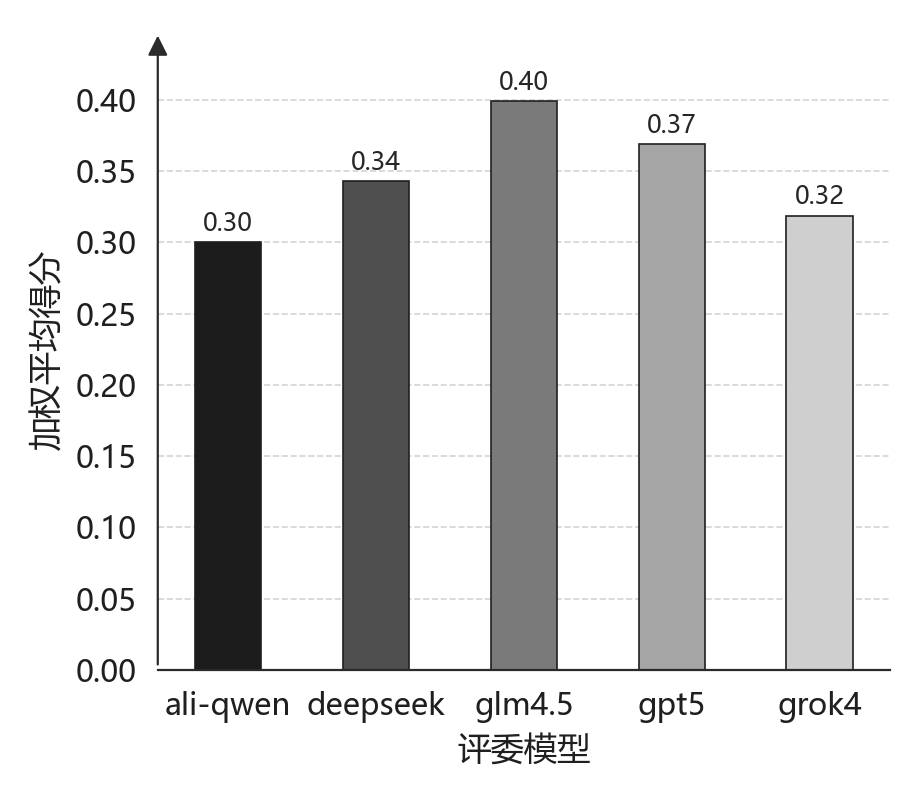
\includegraphics[width=0.95\textwidth]{images/plots/有效性/generator/ali-qwen/generator_bar_by_judge_ali-qwen_有效性.png}}\\
	 \subfloat[\texttt{DeepSeek}\label{fig:app-eff-generator-by-judge-deepseek}]{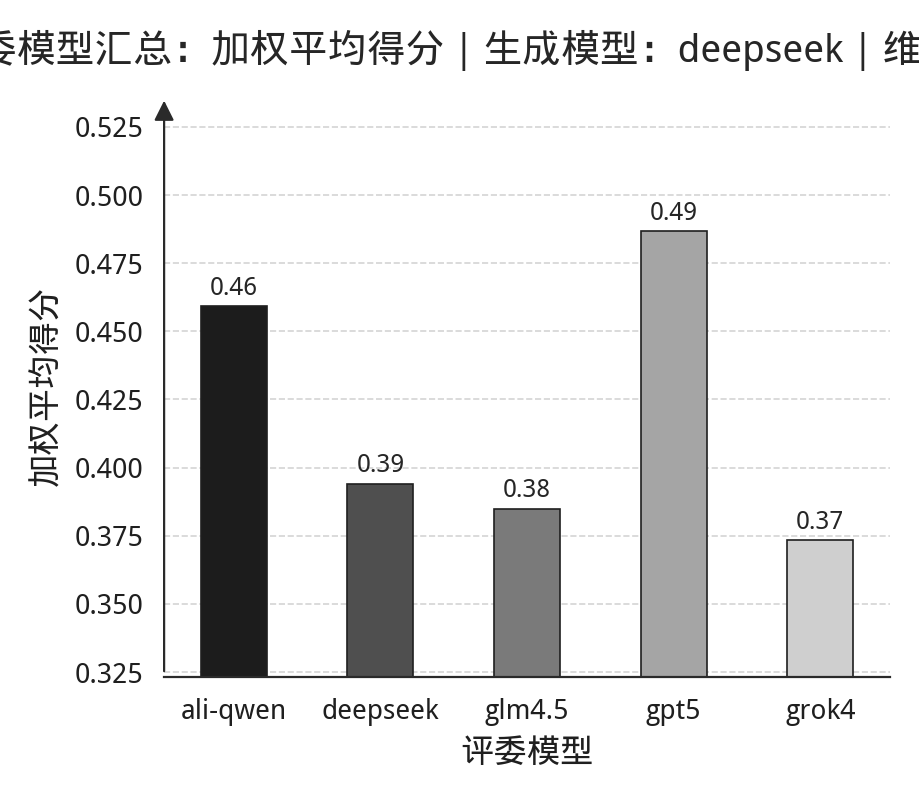
\includegraphics[width=0.95\textwidth]{images/plots/有效性/generator/deepseek/generator_bar_by_judge_deepseek_有效性.png}}\\
	 \subfloat[\texttt{GPT-5}\label{fig:app-eff-generator-by-judge-gpt5}]{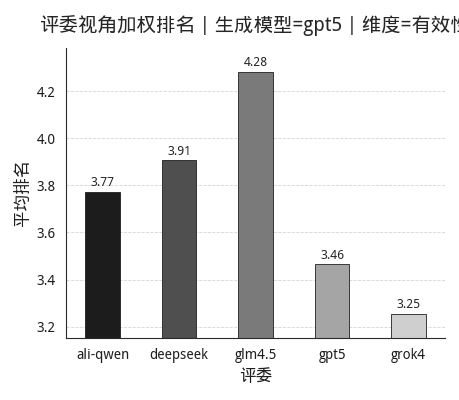
\includegraphics[width=0.95\textwidth]{images/plots/有效性/generator/gpt5/generator_bar_by_judge_gpt5_有效性.png}}}
	\caption{有效性维度下，不同生成模型在各评审模型下的排名式评分对照（I）。}\label{fig:app-eff-generator-by-judge}
\end{figure}

\begin{figure}[!ht]
	\centering
	{\setlength{\abovecaptionskip}{2pt}%
	 \setlength{\belowcaptionskip}{0pt}%
	 \subfloat[\texttt{Grok}\label{fig:app-eff-generator-by-judge-grok}]{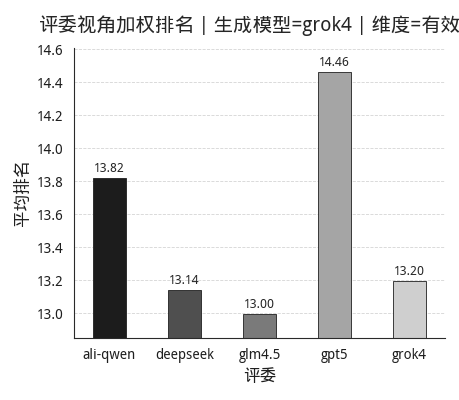
\includegraphics[width=0.95\textwidth]{images/plots/有效性/generator/grok4/generator_bar_by_judge_grok4_有效性.png}}\\
	 \subfloat[\texttt{GLM-4.6}\label{fig:app-eff-generator-by-judge-glm46}]{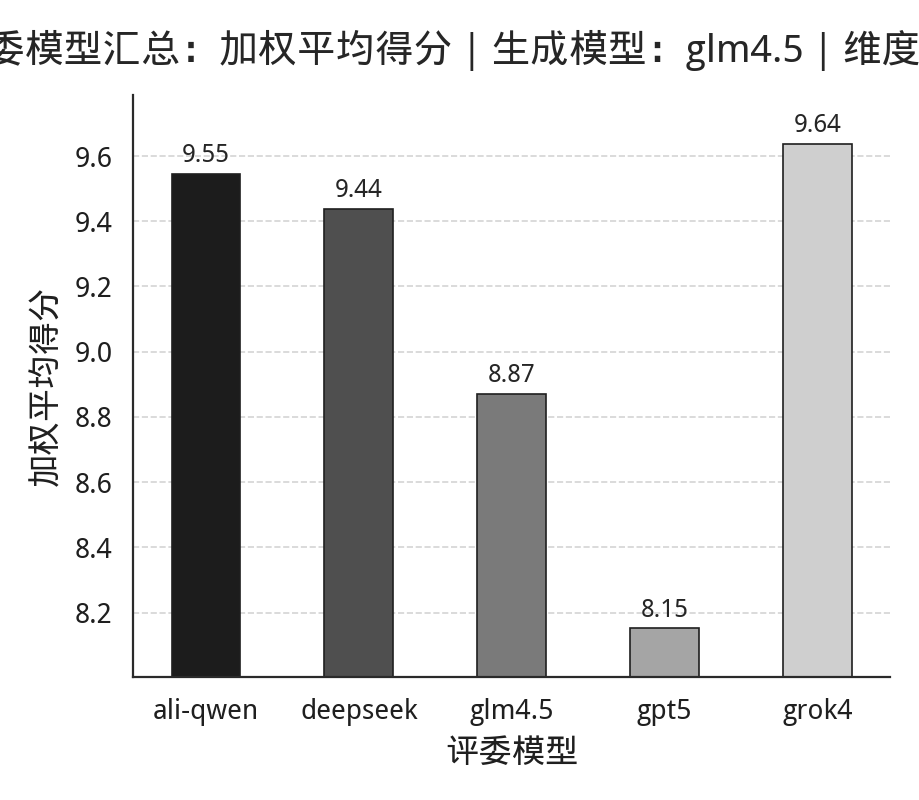
\includegraphics[width=0.95\textwidth]{images/plots/有效性/generator/glm4.5/generator_bar_by_judge_glm4.5_有效性.png}}}
	\caption{有效性维度下，不同生成模型在各评审模型下的排名式评分对照（II）。}\label{fig:app-eff-generator-by-judge-cont}
\end{figure}

\subsection{不同生成模型的结构性对照（热力图）}
\begin{figure}[!ht]
	\centering
	{\setlength{\abovecaptionskip}{2pt}%
	 \setlength{\belowcaptionskip}{0pt}%
	 \subfloat[\texttt{Qwen3}\label{fig:app-eff-heatmap-generator-qwen3}]{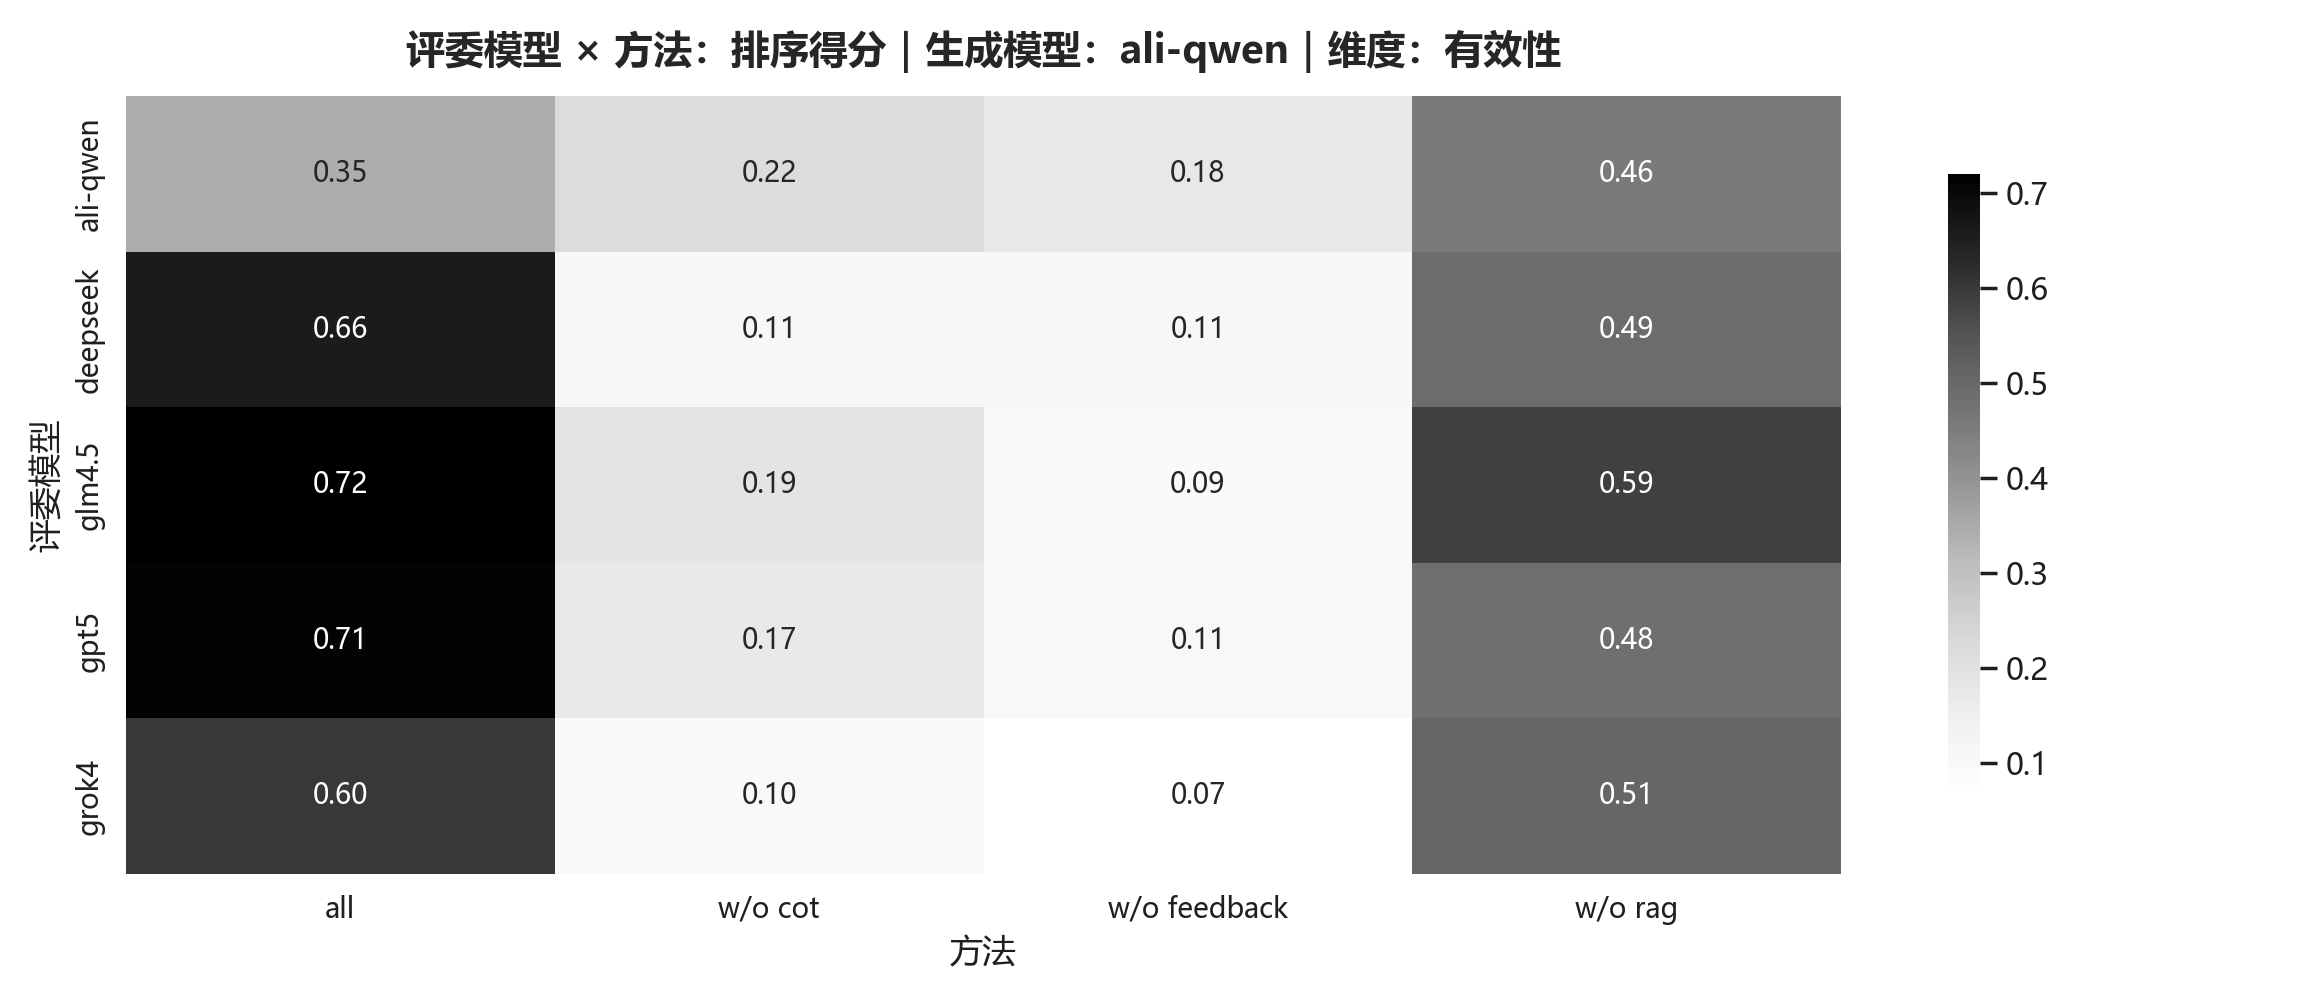
\includegraphics[width=0.95\textwidth]{images/plots/有效性/generator/ali-qwen/heatmap_generator_ali-qwen_有效性.png}}\\
	 \subfloat[\texttt{DeepSeek}\label{fig:app-eff-heatmap-generator-deepseek}]{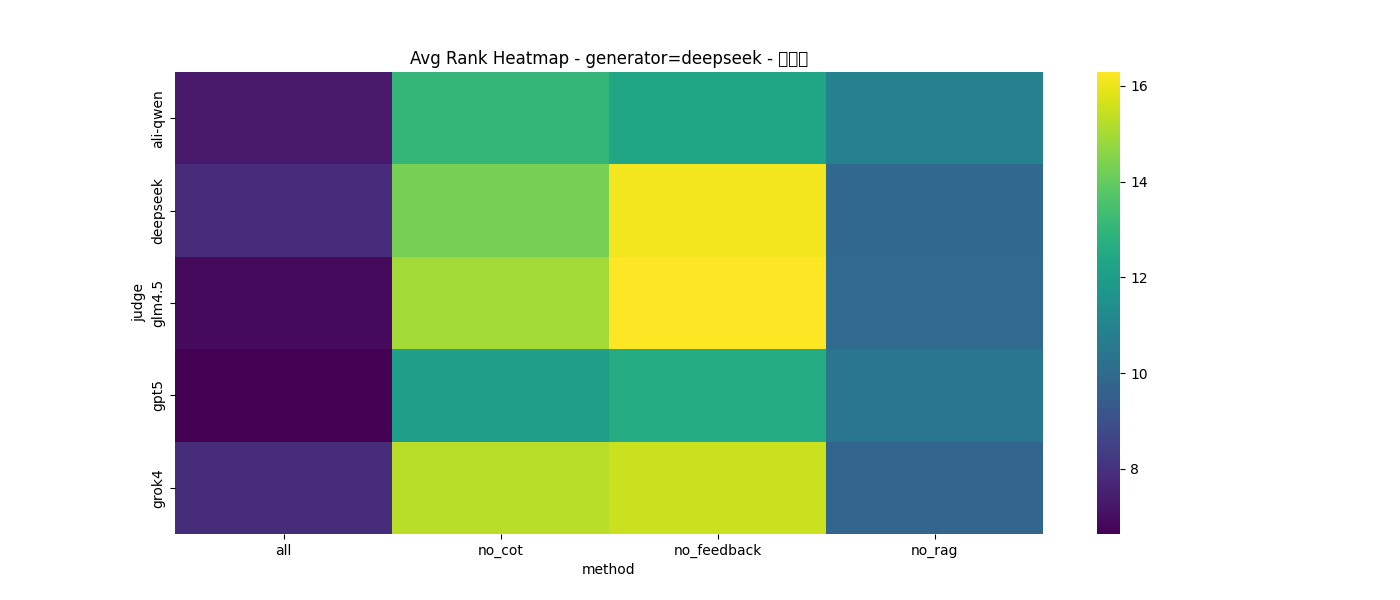
\includegraphics[width=0.95\textwidth]{images/plots/有效性/generator/deepseek/heatmap_generator_deepseek_有效性.png}}\\
	 \subfloat[\texttt{GPT-5}\label{fig:app-eff-heatmap-generator-gpt5}]{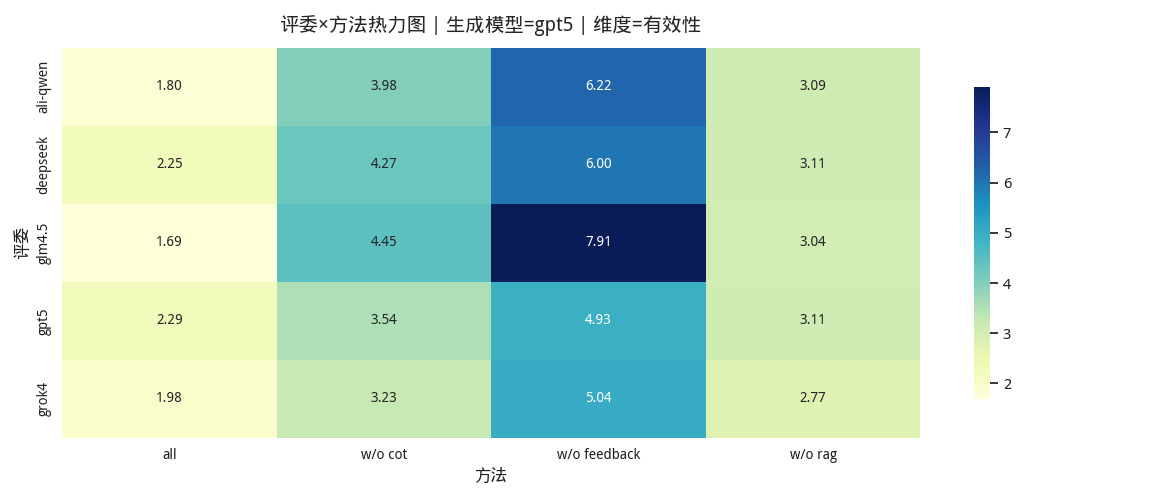
\includegraphics[width=0.95\textwidth]{images/plots/有效性/generator/gpt5/heatmap_generator_gpt5_有效性.png}}}
	\caption{有效性维度下，不同生成模型的结构性热力图对照（I）。}\label{fig:app-eff-heatmap-generator}
\end{figure}

\begin{figure}[!ht]
	\centering
	{\setlength{\abovecaptionskip}{2pt}%
	 \setlength{\belowcaptionskip}{0pt}%
	 \subfloat[\texttt{Grok}\label{fig:app-eff-heatmap-generator-grok}]{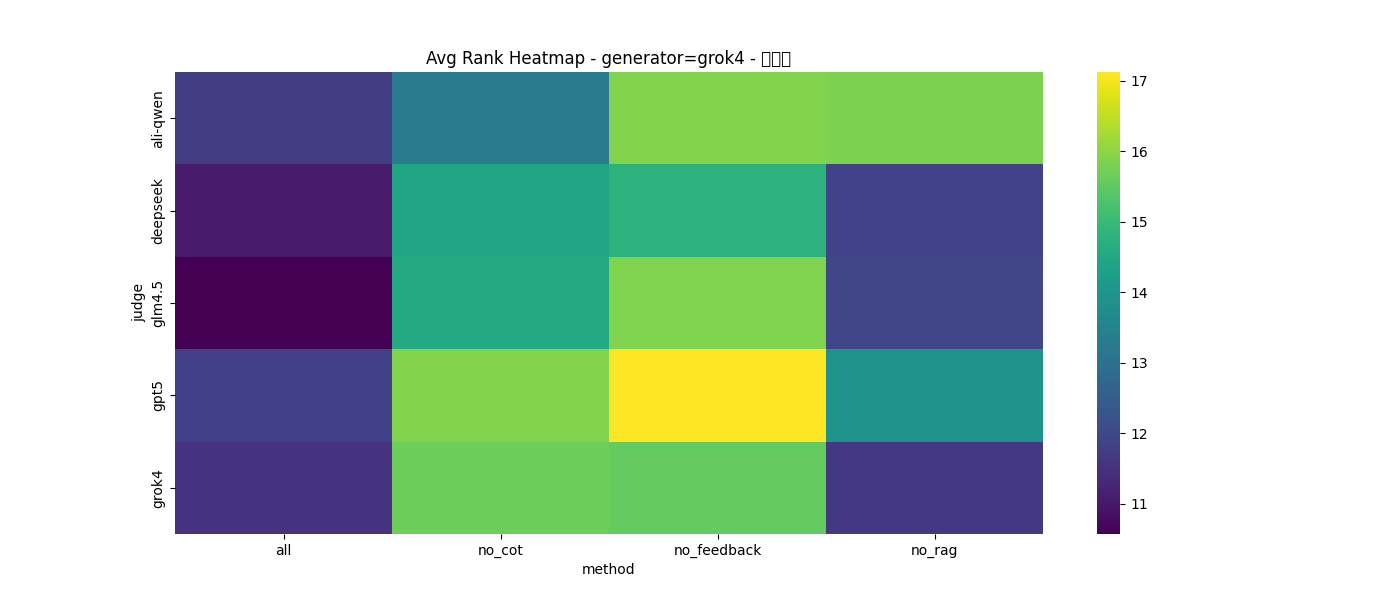
\includegraphics[width=0.95\textwidth]{images/plots/有效性/generator/grok4/heatmap_generator_grok4_有效性.png}}\\
	 \subfloat[\texttt{GLM-4.6}\label{fig:app-eff-heatmap-generator-glm46}]{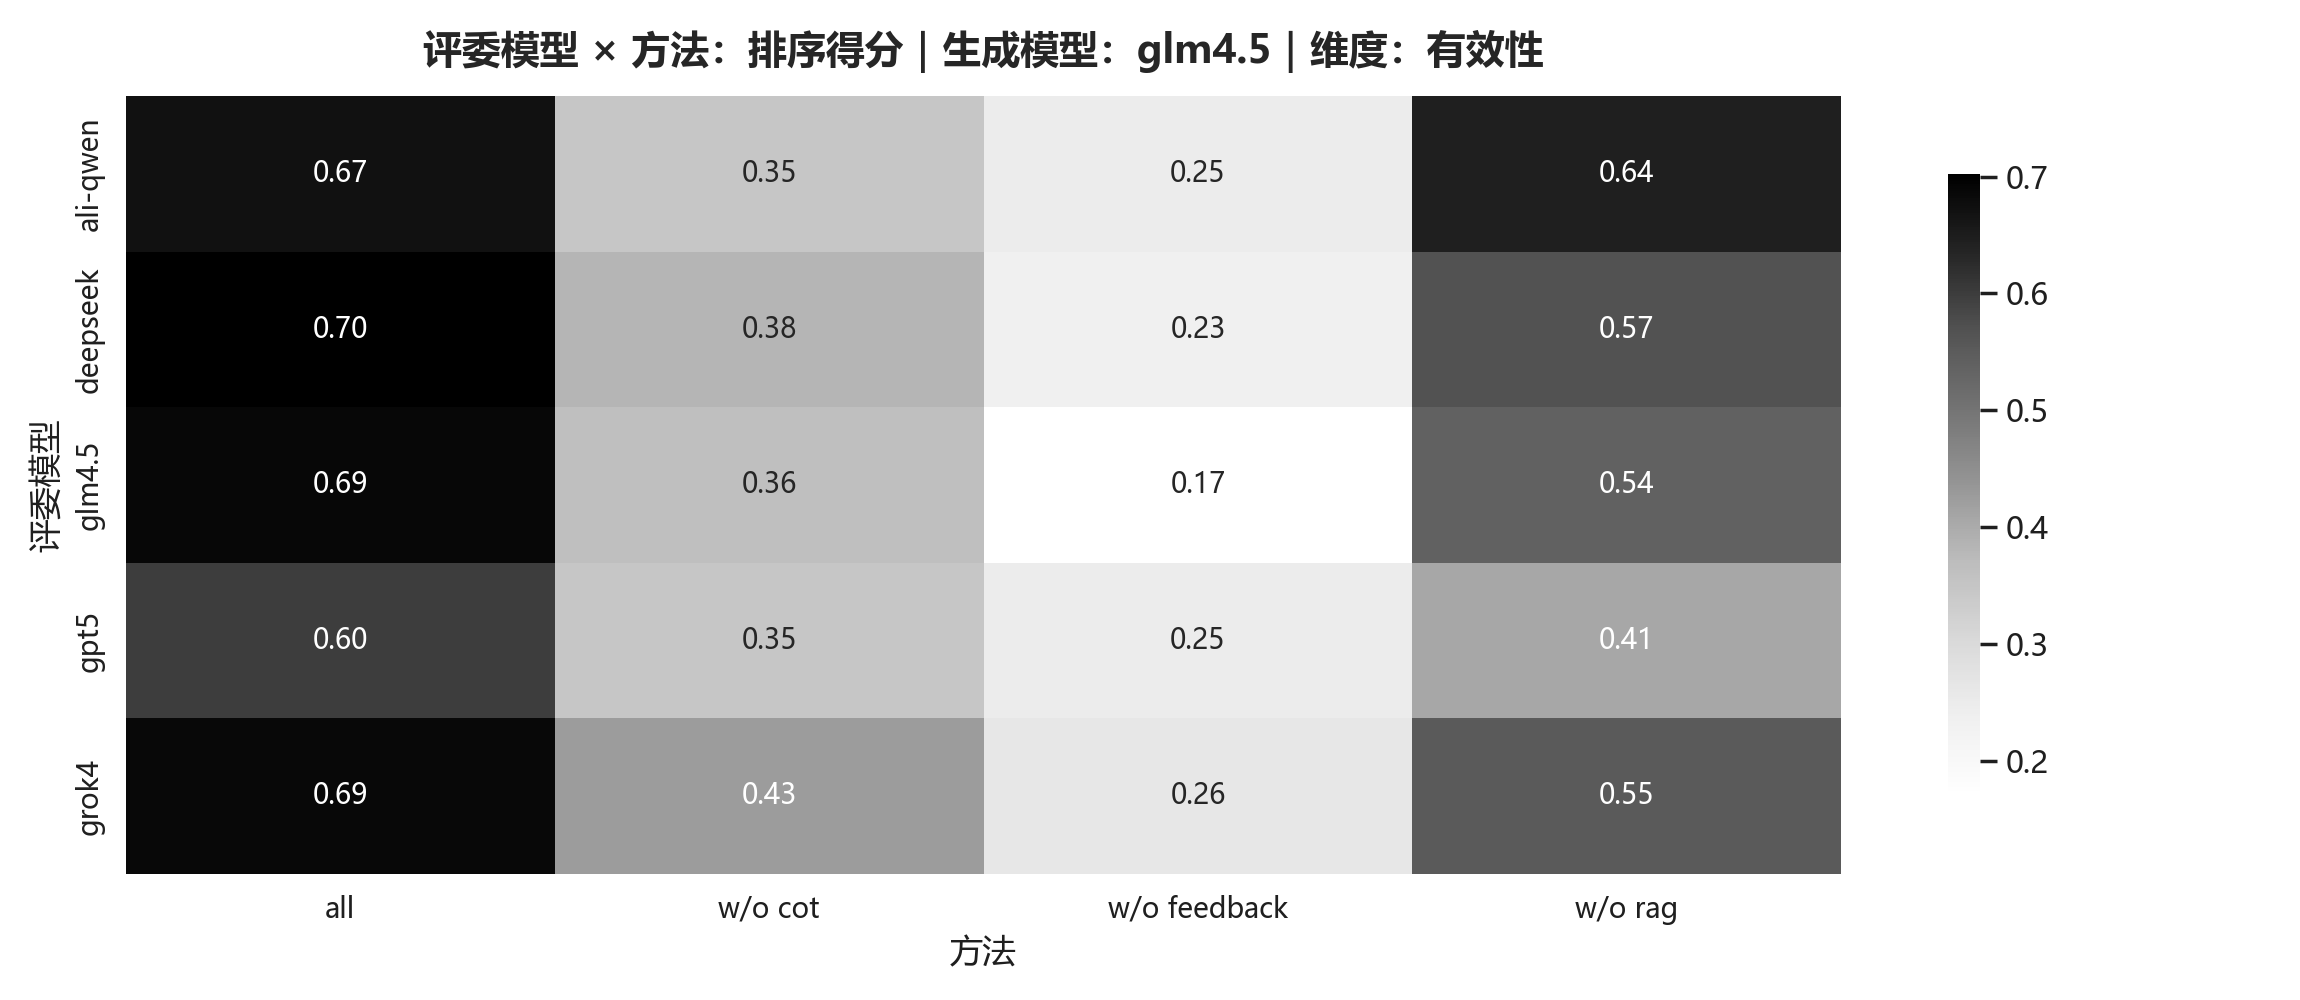
\includegraphics[width=0.95\textwidth]{images/plots/有效性/generator/glm4.5/heatmap_generator_glm4.5_有效性.png}}}
	\caption{有效性维度下，不同生成模型的结构性热力图对照（II）。}\label{fig:app-eff-heatmap-generator-cont}
\end{figure}

\section{可部署性：补充图表}\label{app:plots-deployability}

\subsection{按生成模型拆分的热力图（评审偏好结构）}
\begin{figure}[!ht]
	\centering
	{\setlength{\abovecaptionskip}{2pt}%
	 \setlength{\belowcaptionskip}{0pt}%
	 \subfloat[\texttt{Qwen3}\label{fig:app-deploy-heatmap-qwen3}]{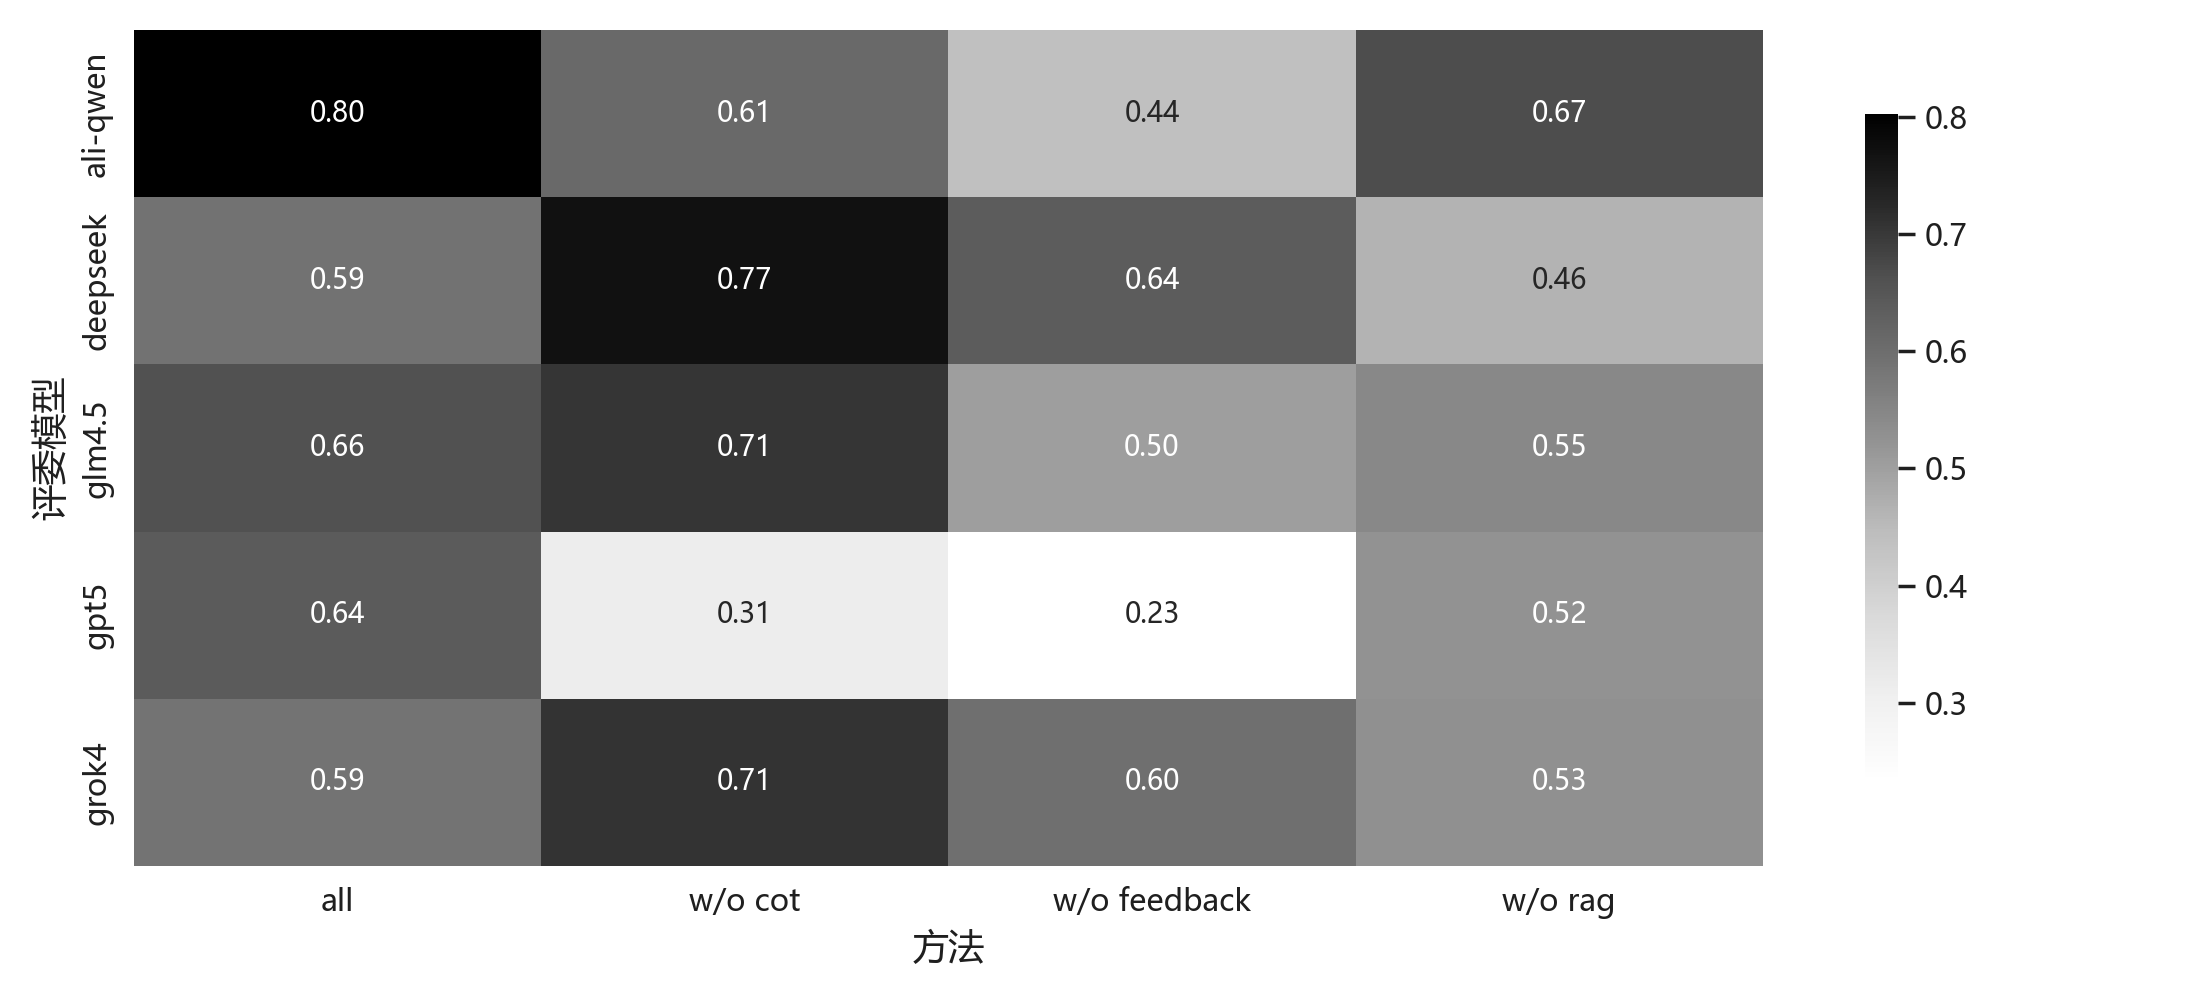
\includegraphics[width=0.95\textwidth]{images/plots/可部署性/heatmap/ali-qwen/heatmap_ali-qwen_可部署性.png}}\\
	 \subfloat[\texttt{DeepSeek}\label{fig:app-deploy-heatmap-deepseek}]{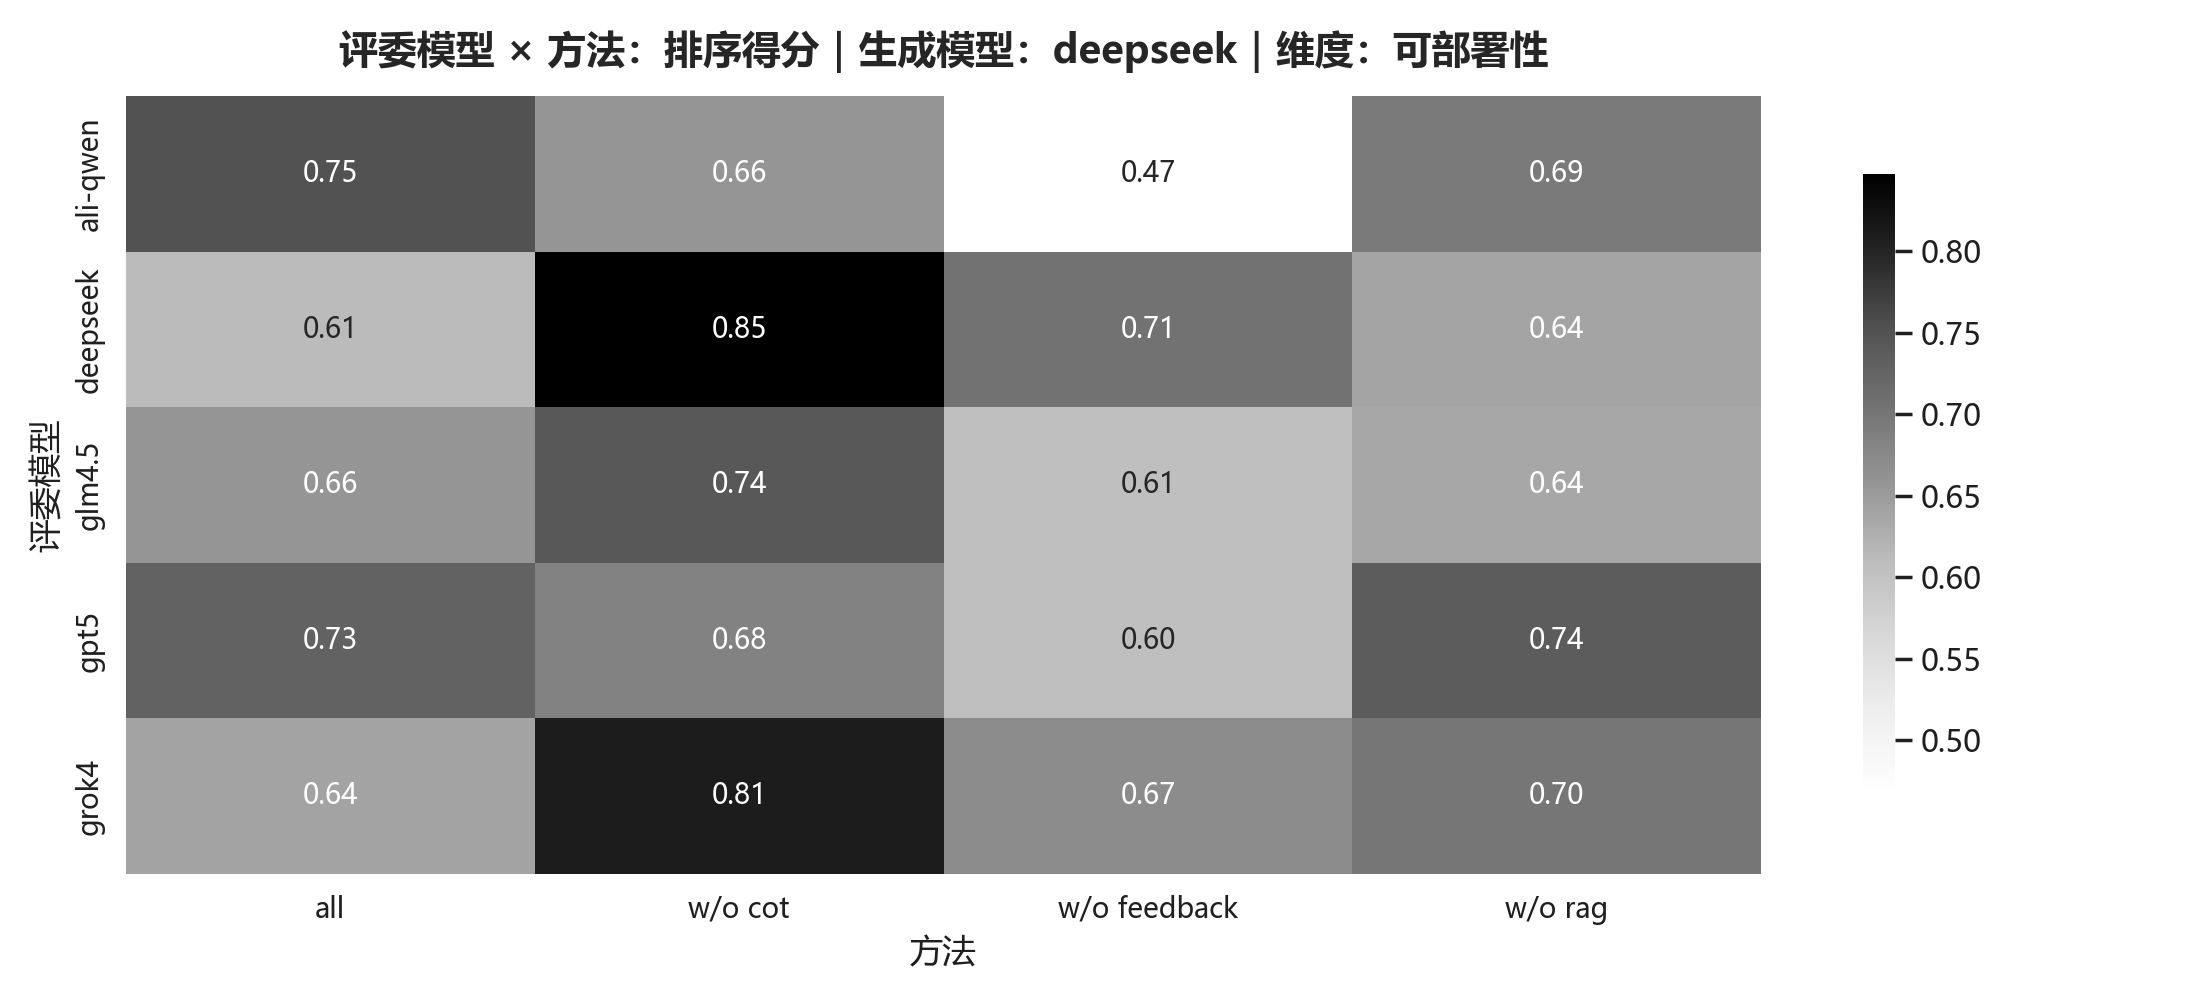
\includegraphics[width=0.95\textwidth]{images/plots/可部署性/heatmap/deepseek/heatmap_deepseek_可部署性.png}}\\
	 \subfloat[\texttt{GPT-5}\label{fig:app-deploy-heatmap-gpt5}]{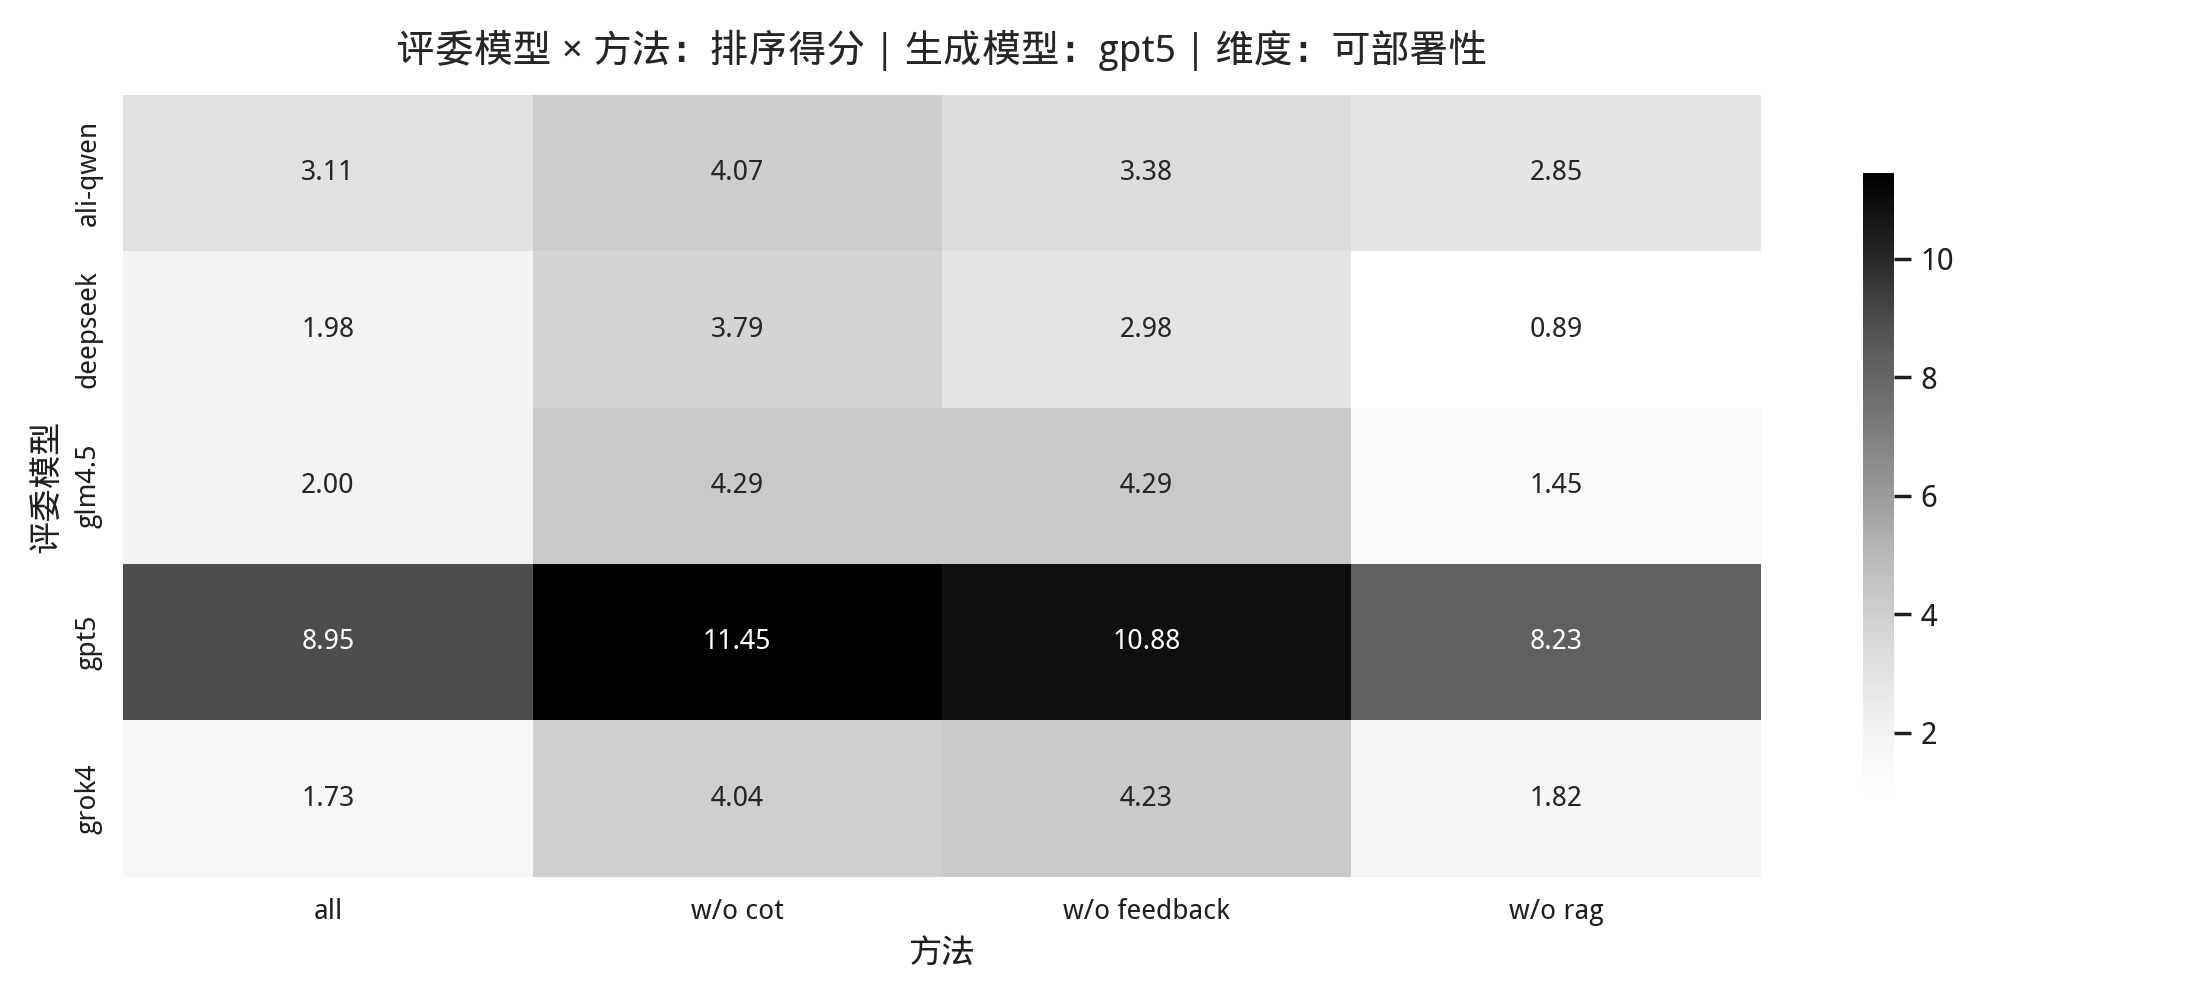
\includegraphics[width=0.95\textwidth]{images/plots/可部署性/heatmap/gpt5/heatmap_gpt5_可部署性.png}}}
	\caption{可部署性维度下，不同评审模型的偏好结构热力图对照（I）。}\label{fig:app-deploy-heatmap}
\end{figure}

\begin{figure}[!ht]
	\centering
	{\setlength{\abovecaptionskip}{2pt}%
	 \setlength{\belowcaptionskip}{0pt}%
	 \subfloat[\texttt{Grok}\label{fig:app-deploy-heatmap-grok}]{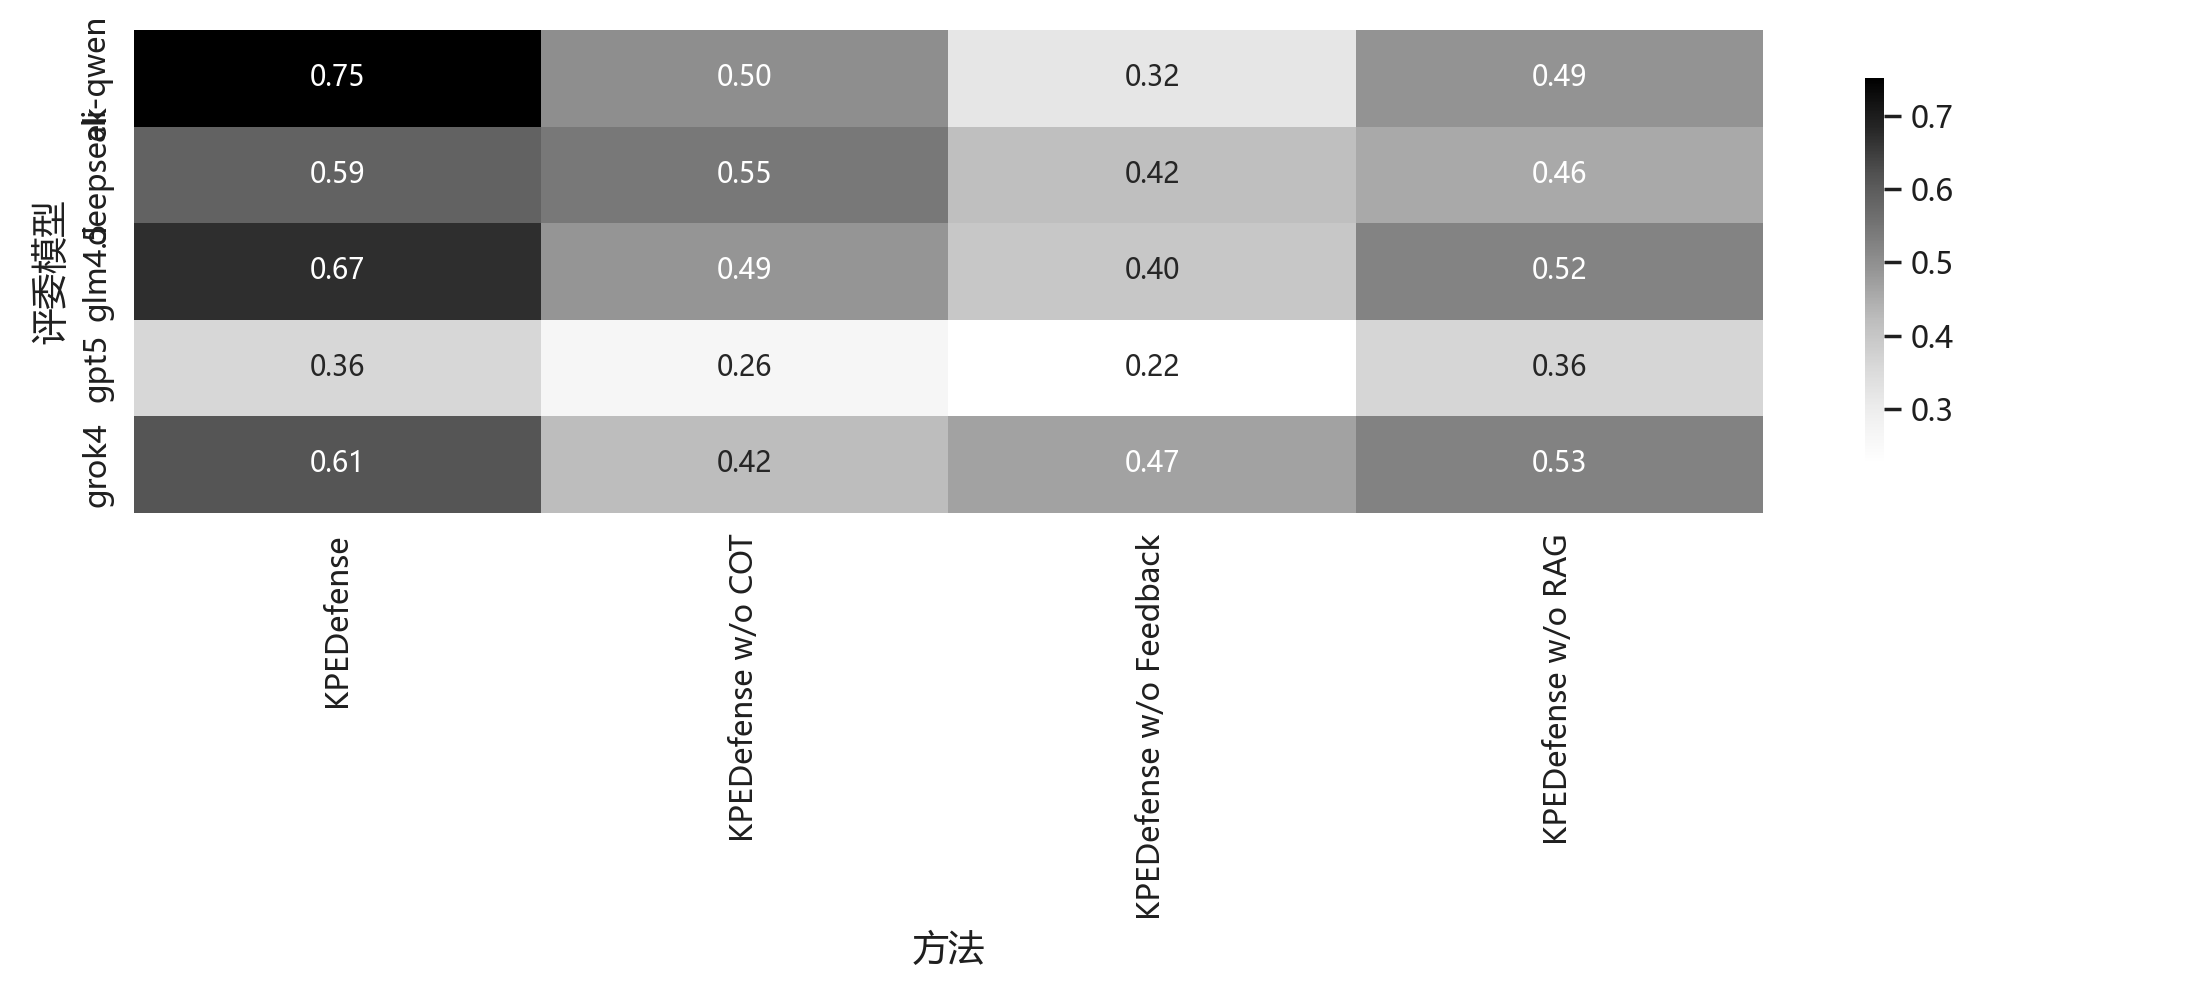
\includegraphics[width=0.95\textwidth]{images/plots/可部署性/heatmap/grok4/heatmap_grok4_可部署性.png}}\\
	 \subfloat[\texttt{GLM-4.6}\label{fig:app-deploy-heatmap-glm46}]{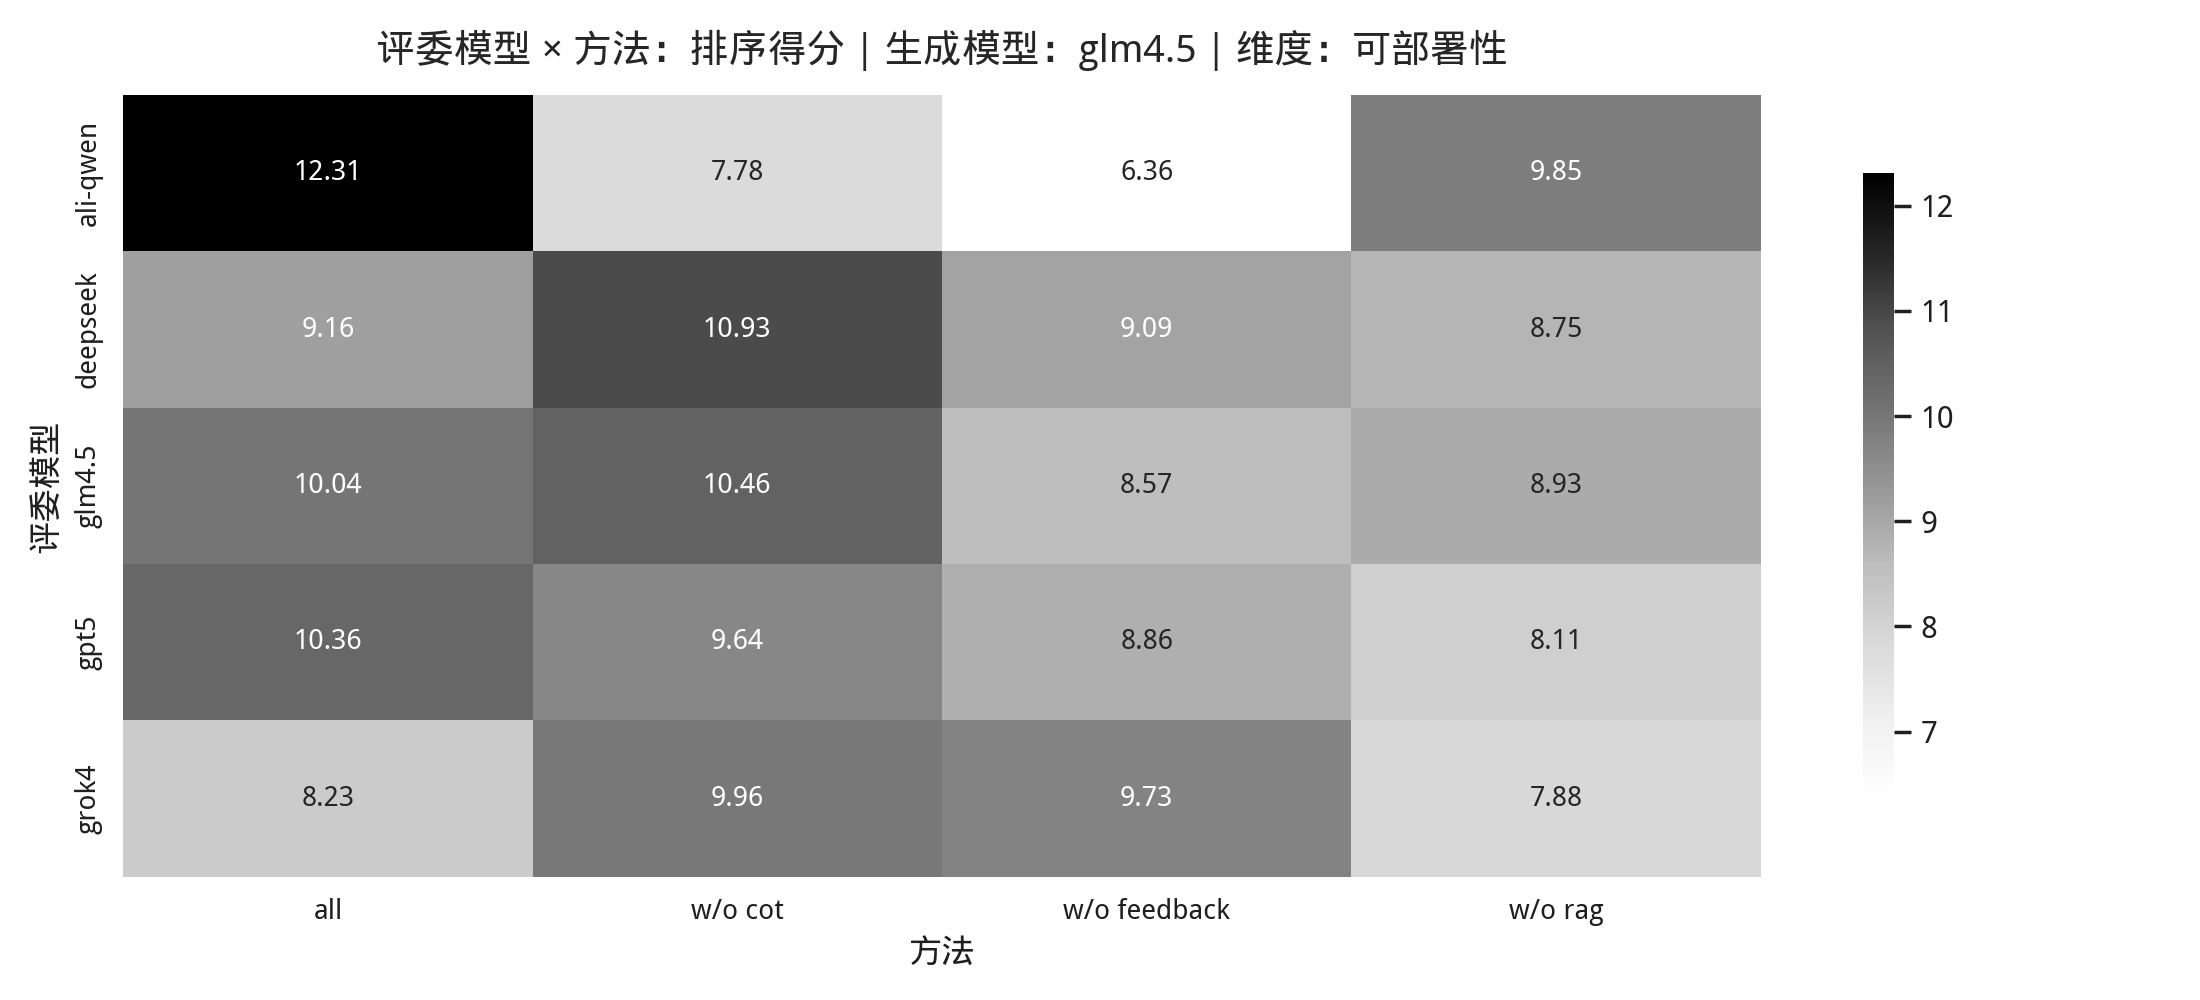
\includegraphics[width=0.95\textwidth]{images/plots/可部署性/heatmap/glm4.5/heatmap_glm4.5_可部署性.png}}}
	\caption{可部署性维度下，不同评审模型的偏好结构热力图对照（II）。}\label{fig:app-deploy-heatmap-cont}
\end{figure}

\section{无干扰性：补充图表}\label{app:plots-interference}

\subsection{按生成模型拆分的热力图（评审偏好结构）}
\begin{figure}[!ht]
	\centering
	{\setlength{\abovecaptionskip}{2pt}%
	 \setlength{\belowcaptionskip}{0pt}%
	 \subfloat[\texttt{Qwen3}\label{fig:app-interf-heatmap-qwen3}]{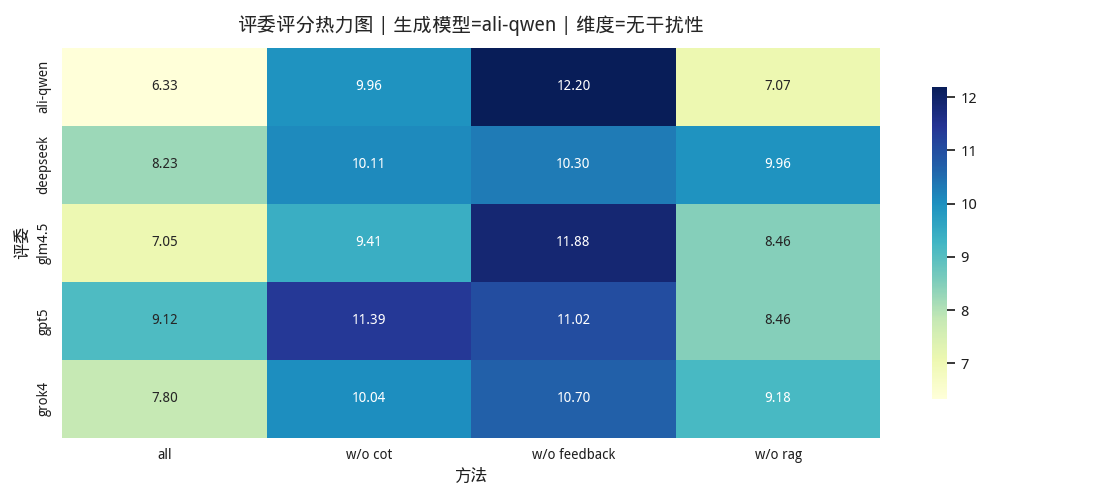
\includegraphics[width=0.95\textwidth]{images/plots/无干扰性/heatmap/ali-qwen/heatmap_ali-qwen_无干扰性.png}}\\
	 \subfloat[\texttt{DeepSeek}\label{fig:app-interf-heatmap-deepseek}]{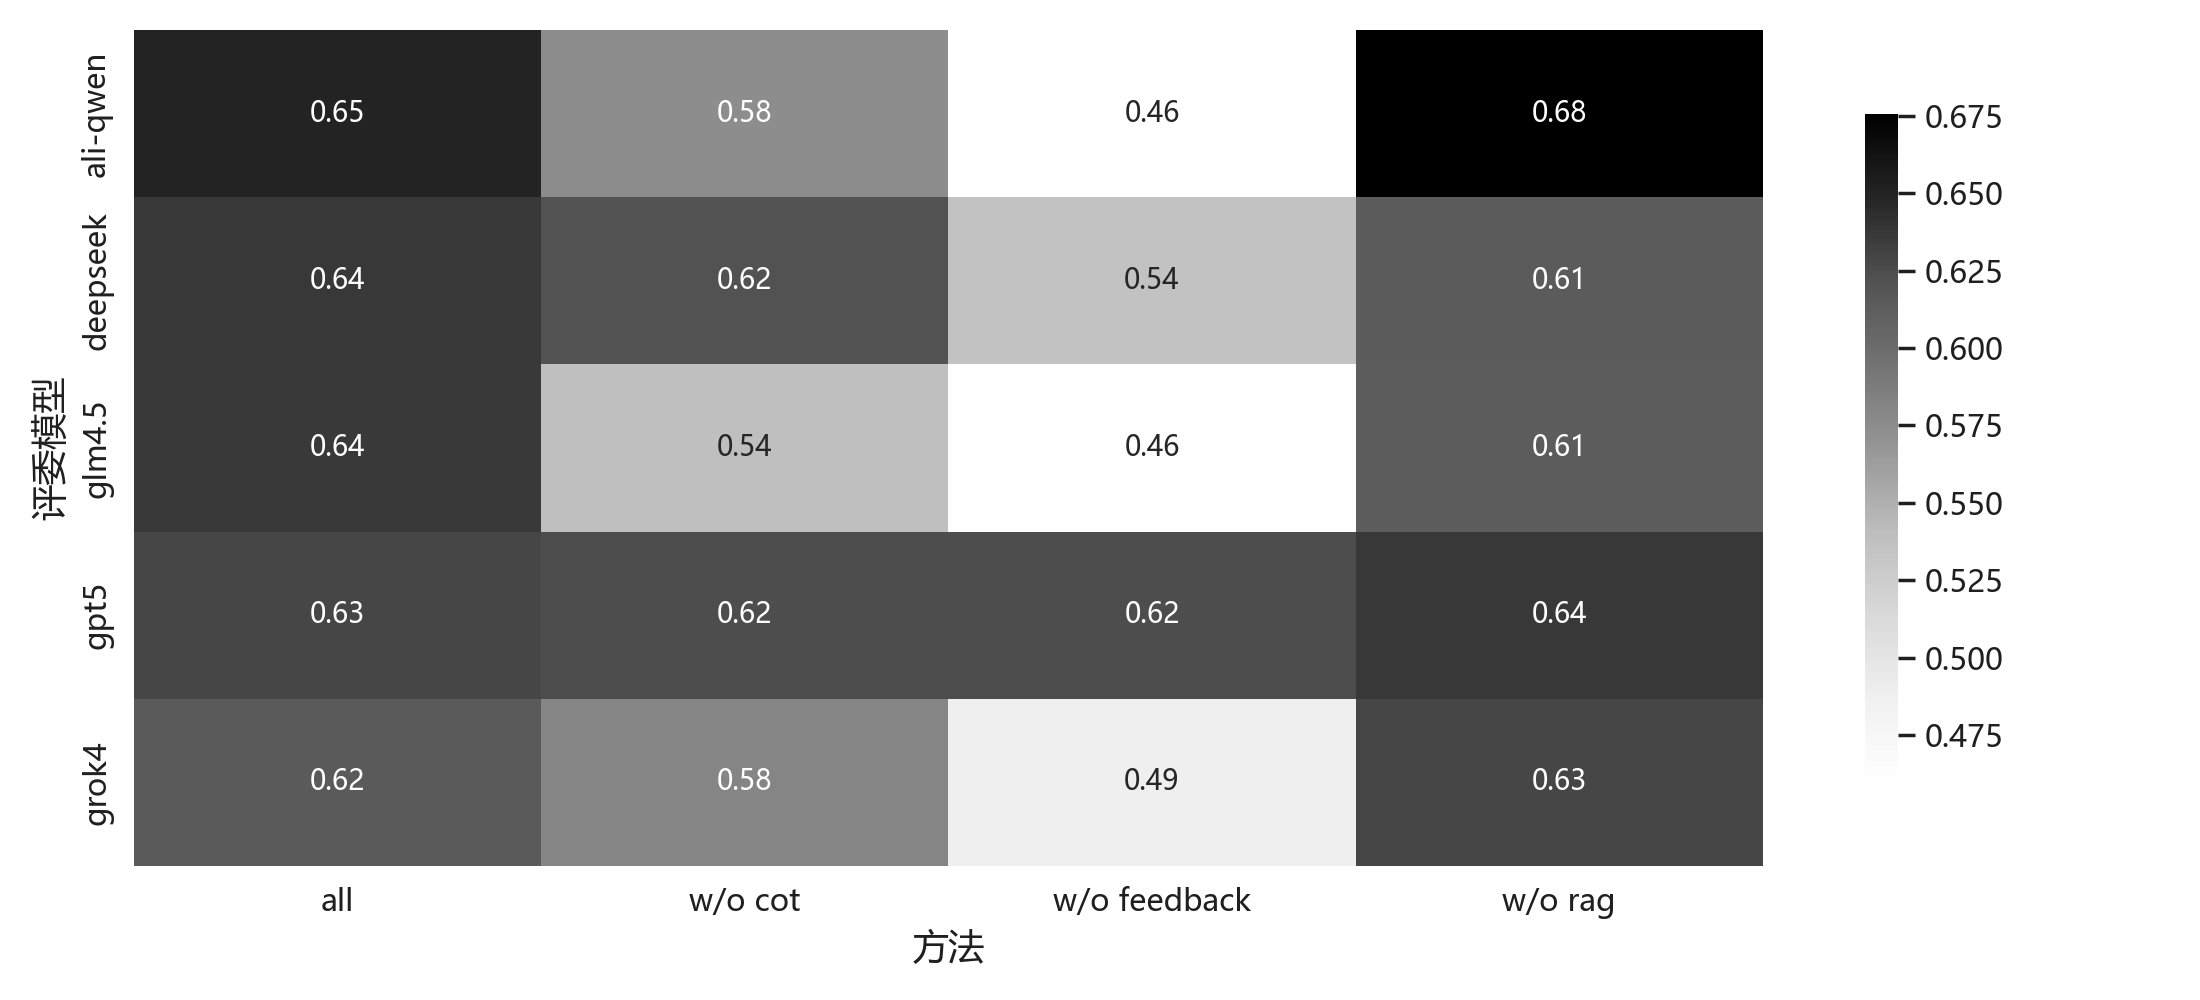
\includegraphics[width=0.95\textwidth]{images/plots/无干扰性/heatmap/deepseek/heatmap_deepseek_无干扰性.png}}\\
	 \subfloat[\texttt{GPT-5}\label{fig:app-interf-heatmap-gpt5}]{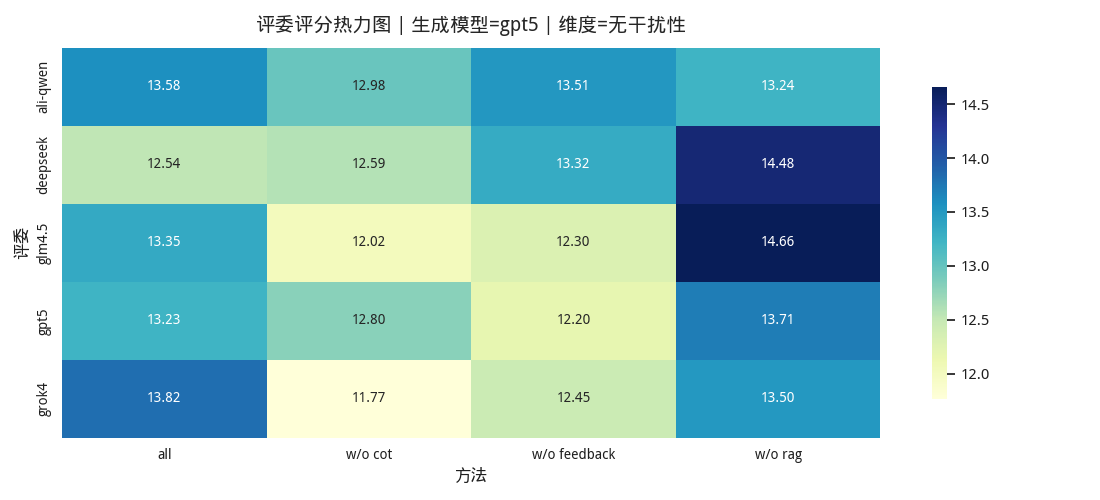
\includegraphics[width=0.95\textwidth]{images/plots/无干扰性/heatmap/gpt5/heatmap_gpt5_无干扰性.png}}}
	\caption{无干扰性维度下，不同评审模型的偏好结构热力图对照（I）。}\label{fig:app-interf-heatmap}
\end{figure}

\begin{figure}[!ht]
	\centering
	{\setlength{\abovecaptionskip}{2pt}%
	 \setlength{\belowcaptionskip}{0pt}%
	 \subfloat[\texttt{Grok}\label{fig:app-interf-heatmap-grok}]{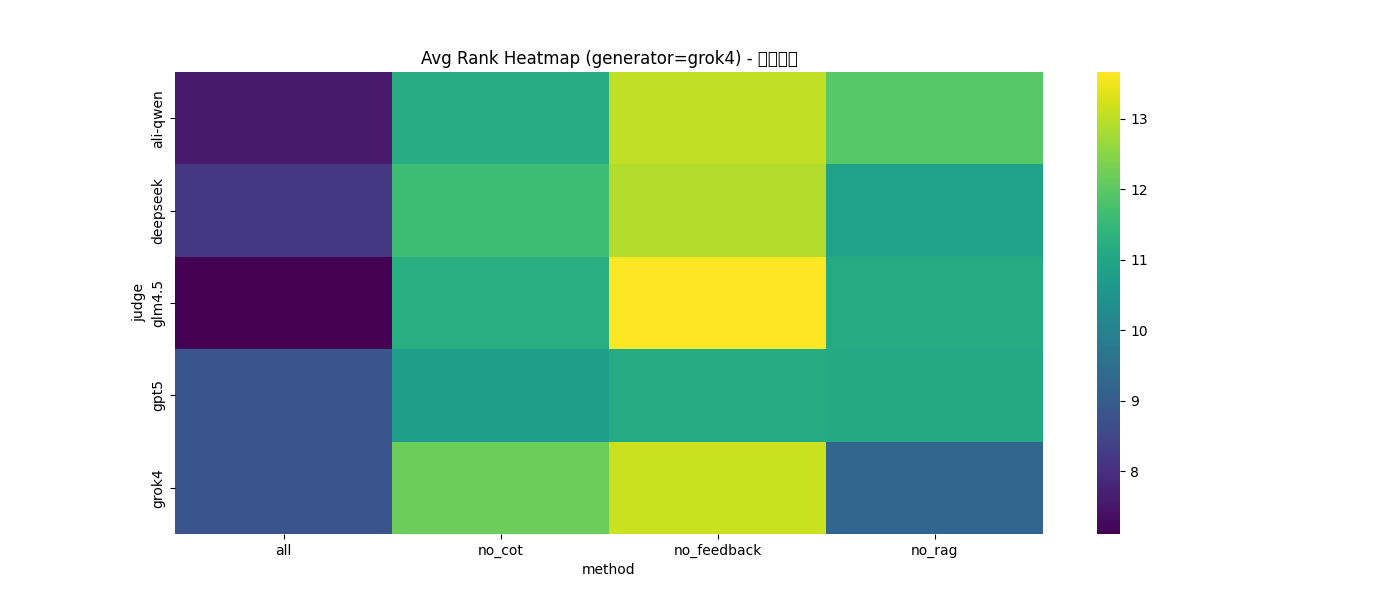
\includegraphics[width=0.95\textwidth]{images/plots/无干扰性/heatmap/grok4/heatmap_grok4_无干扰性.png}}\\
	 \subfloat[\texttt{GLM-4.6}\label{fig:app-interf-heatmap-glm46}]{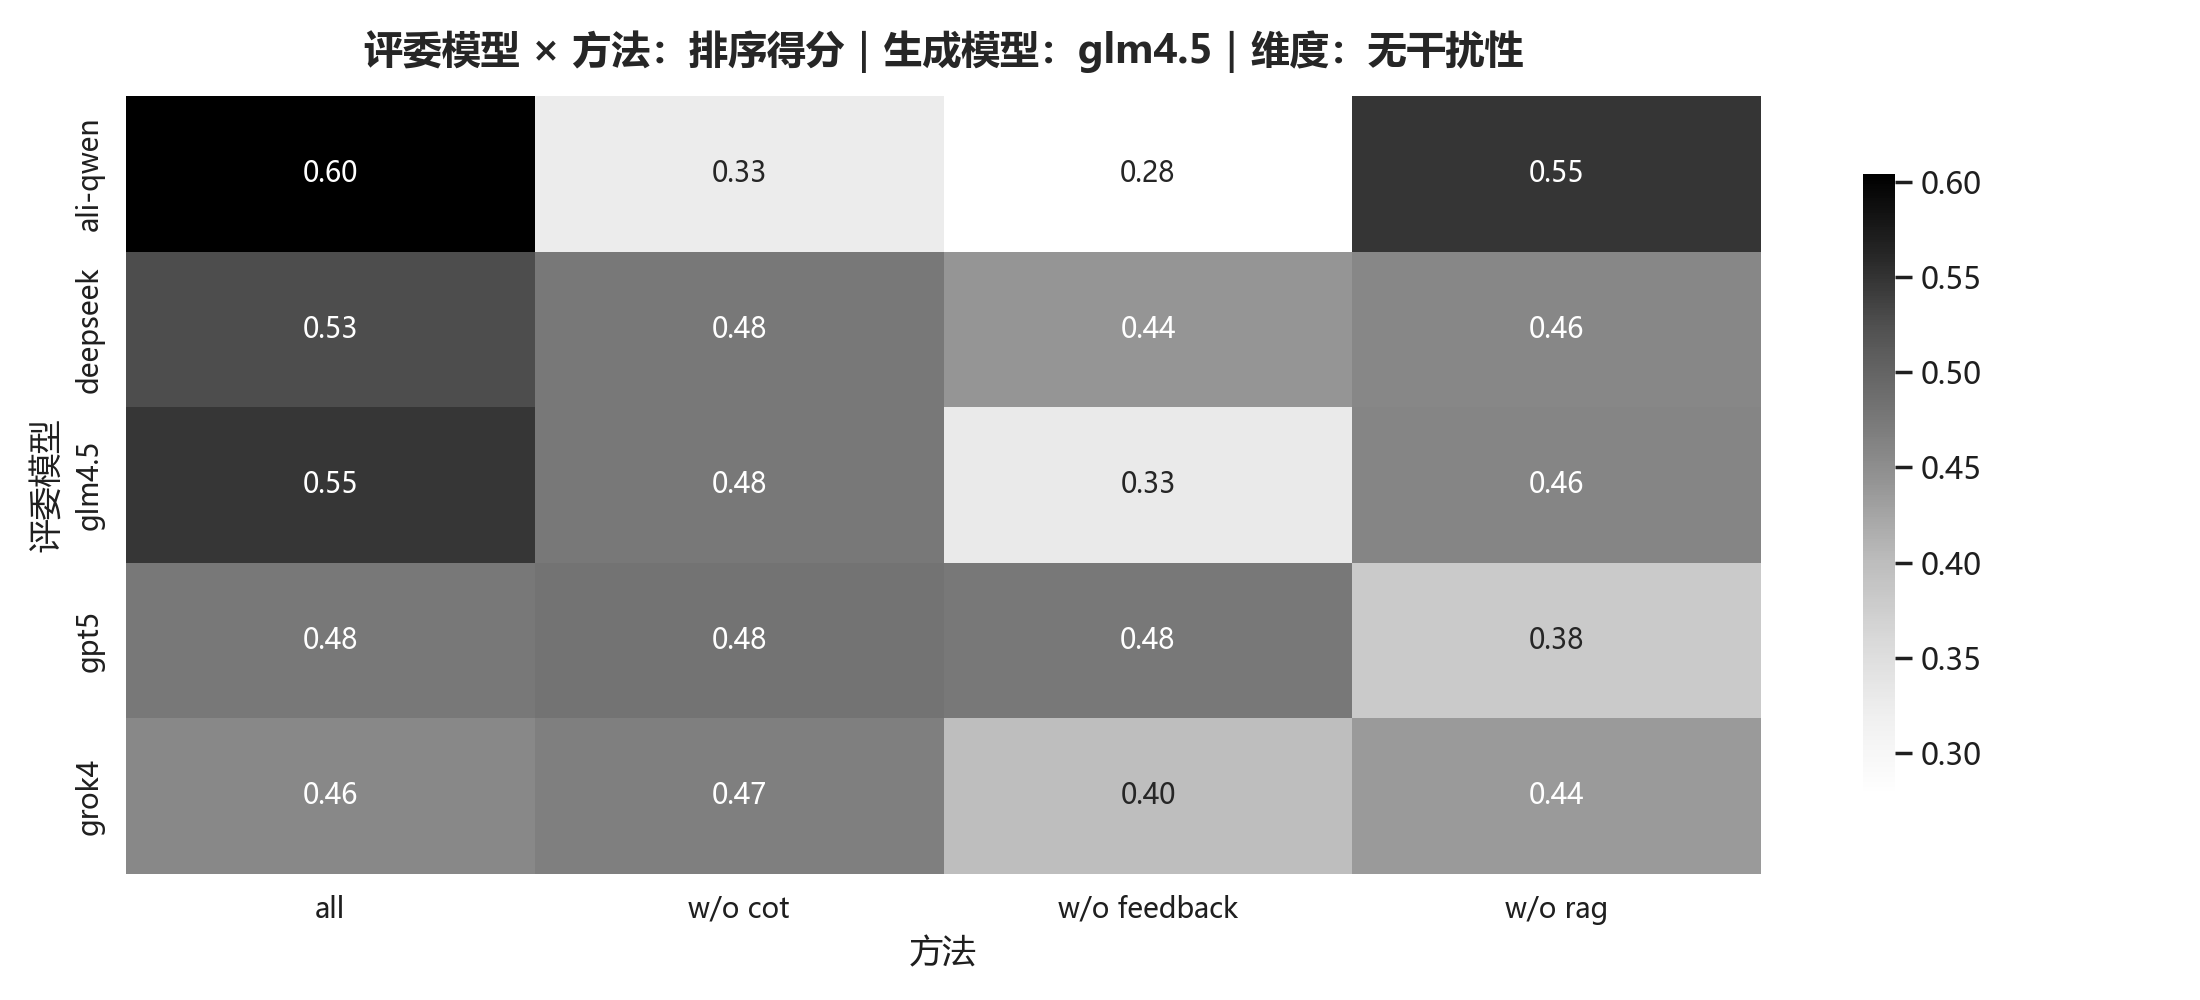
\includegraphics[width=0.95\textwidth]{images/plots/无干扰性/heatmap/glm4.5/heatmap_glm4.5_无干扰性.png}}}
	\caption{无干扰性维度下，不同评审模型的偏好结构热力图对照（II）。}\label{fig:app-interf-heatmap-cont}
\end{figure}